\section{Background and Related Works}
\subsection{LLM Search Agent}
\begin{figure}[t]
    \centering
    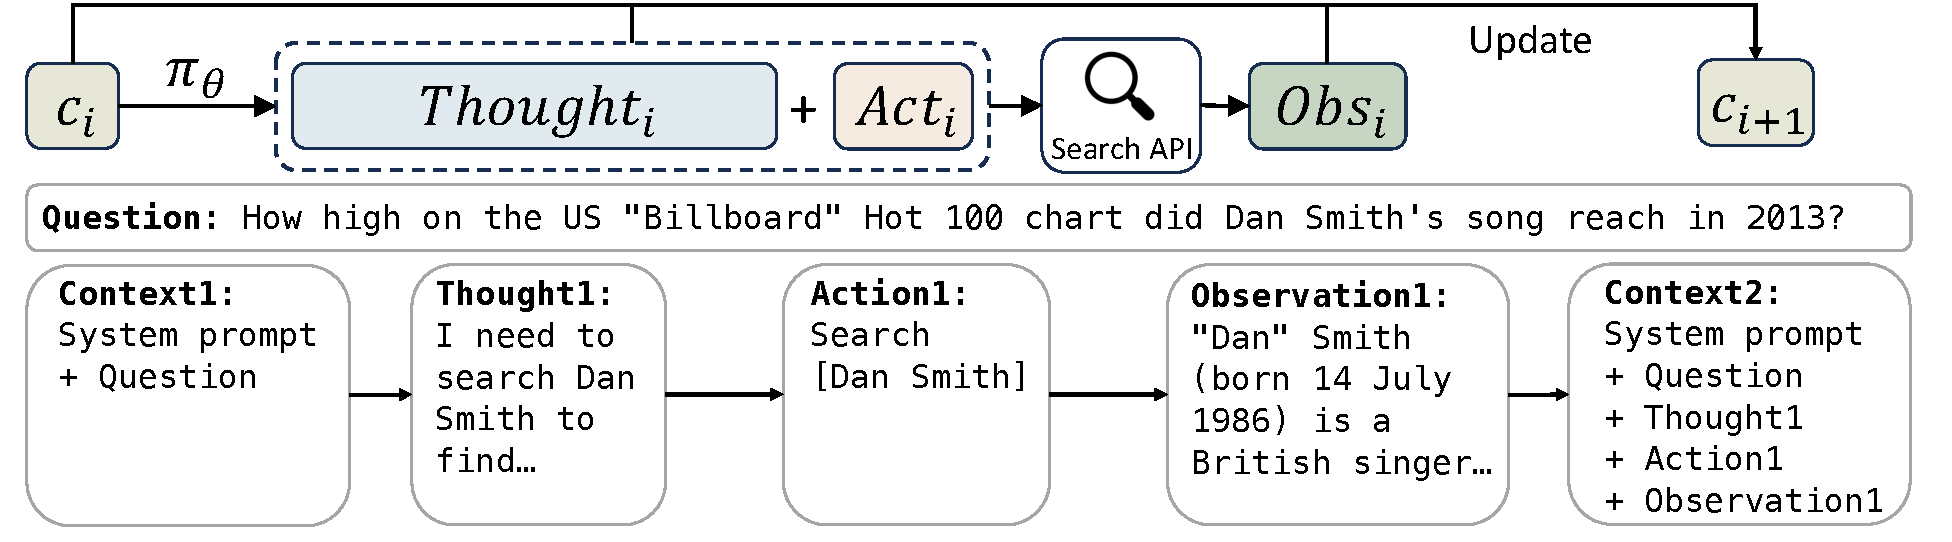
\includegraphics[width=0.95\linewidth]{figures/naive_path.pdf}
    % \vspace{-10pt}
    \caption{Naive ReAct search agent~\cite{react}}
    \label{fig:naive_step}
    % \vspace{-10pt}
\end{figure}

Across the evolution of LLM-based search agents, from workflow-level design~\cite{lats,search-o1} to agents recently trained via reinforcement learning ~\cite{search-r1,ReSearch}, the iterative reason-action has emerged as the de facto standard for evidence collection and decision refinement.
A typical search agent for task solving is shown in \Figref{fig:naive_step}.
At step $i$, the agent maintains a context $c_i$ containing the system prompt along with all previous thoughts, actions, and observations (result of action execution). 
Given $c_i$, the agent generates both a reasoning content $Thought_i$ and an action $Act_i$ by an inference call ($\pi_\theta$) for the current step. 
The action is then executed via the external tools (e.g., search API), yielding an observation that is appended to the context to form $c_{i+1}$. 
This loop continues until the agent generates a final answer and terminates the task.
Under this paradigm, model inference and action execution form a strictly serial dependency, which is the fundamental cause of the high latency in search agents.

\subsection{Speculative Decoding}
Speculative decoding accelerates LLM inference via a predict–verify pipeline, where draft tokens proposed by a smaller model are verified by a larger one~\cite{speculativedecoding,eagle,speculativesampling}.
This reduces decoding latency, but its benefit to search agents is limited because their end-to-end latency is dominated not only by model inference but also by substantial tool-execution time.
Related ideas are being explored in LLM agents.
Works of speculative planning~\cite{speculativeplanning} and speculative actions~\cite{speculativeactions} also follow the predict-verify paradigm.
However, these approaches introduce extra inference requests, which can yield negative effects under high concurrency~\cite{turbospec}.


\subsection{LLM Inference System}
Due to the inherent cost variation in LLM inference~\cite{inferencesurvey}, standard throughput-oriented policies~\cite{vllm,orca} often suffer from head-of-line blocking, where short requests are delayed by long ones. 
This limitation becomes critical in high-concurrency scenarios involving mixed speculative and reasoning requests, necessitating dynamic scheduling to maintain system responsiveness.


